\documentclass[10pt,a4paper]{article}
\usepackage[scale=0.75,a4paper]{geometry}
\usepackage[utf8]{inputenc}
\usepackage{amsmath}
\usepackage{amsfonts}
\usepackage{amssymb}
\usepackage{babel}
\usepackage{graphicx}




\author{Oduwole Eunice}
\title{ Tweet archive of  WeRateDogs (Act Report)}
\begin{document}
\maketitle
%\noindent From the summary statistics we saw that on average, the fist image  prediction has a higher confidence value. 

\begin{figure}[!h]
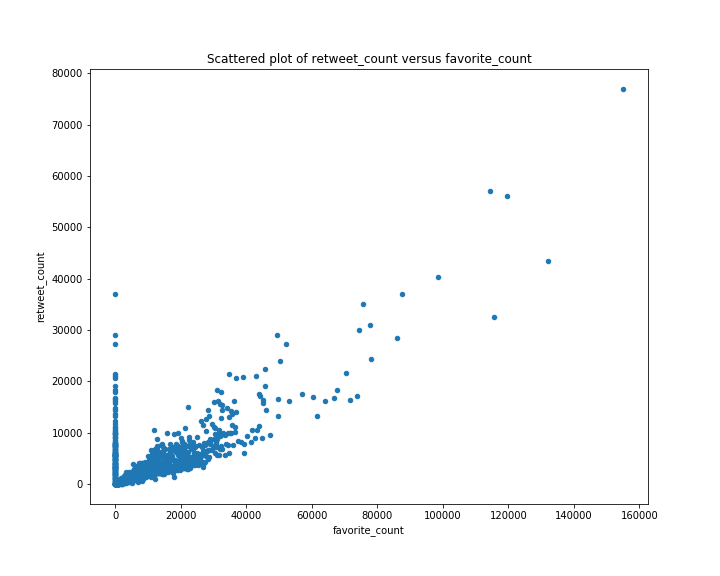
\includegraphics[scale=0.3]{twitter_archiveplot.png} 
\caption{Scattered plot of retweet count versus favorite count}
\label{fig1}
\end{figure}
\noindent From figure  \ref{fig1} there appears to be a positive correlation between favourite and retweet. So we could say as the count of the favorites dogs increases, the more the retweet counts also increases. 

\begin{figure}[!h]
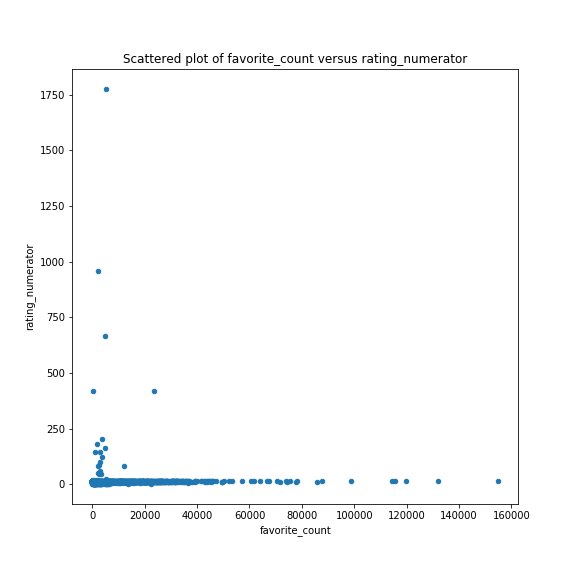
\includegraphics[scale=0.3]{Scattered_numerator.png} 
\caption{Scattered plot of favorite count versus rating numerator}
\label{fig2}
\end{figure}

\noindent From figure  \ref{fig2} there is no correlation between favourite and rating . The rating does not affect the rate at which people like the dogs. 

\newpage

\begin{figure}[!h]
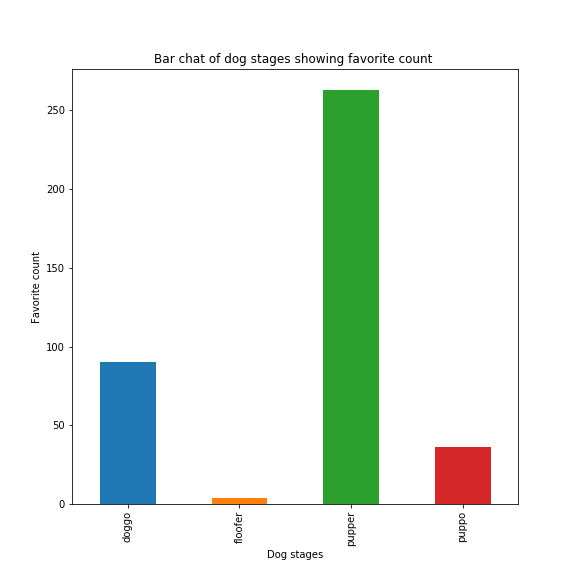
\includegraphics[scale=0.3]{Favorite_count.png} 
\caption{Bar chat of dog stages showing favorite count}
\label{fig3}
\end{figure}
Figure  \ref{fig3} reviews that the dog stage pupper has the highest favorite count. 


\begin{figure}[!h]
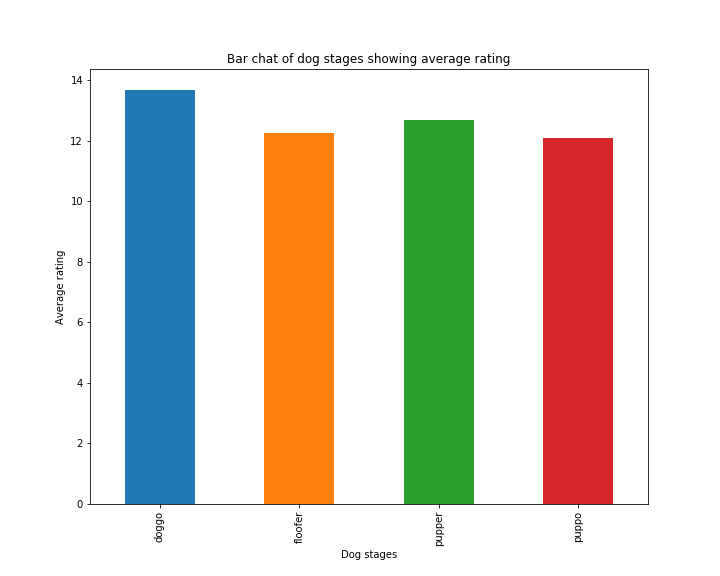
\includegraphics[scale=0.3]{Average_rating.png} 
\caption{Bar chat of dog stages showing average rating}
\label{fig4}
\end{figure}
Figure  \ref{fig4} reviews on average, that the dog stage doggo on  has the highest rating on average. 










\end{document}